\documentclass[12pt]{article}
\usepackage{graphicx}
\usepackage{subcaption}
\usepackage{amsfonts}
\usepackage{amsthm}
\usepackage{amsmath}
\usepackage{blkarray}
\usepackage{multirow}
\usepackage[labelfont=bf]{caption}
\usepackage[margin=1.5in]{geometry}
\usepackage{color}
\usepackage{algorithmic}
\usepackage{algorithm}
\usepackage{listings}

\usepackage{color}

\definecolor{dkgreen}{rgb}{0,0.6,0}
\definecolor{gray}{rgb}{0.5,0.5,0.5}
\definecolor{mauve}{rgb}{0.58,0,0.82}
\definecolor{darkblue}{rgb}{0.0,0.0,0.6}
\definecolor{cyan}{rgb}{0.0,0.6,0.6}

\lstset{frame=tb,
%	language=Python,
	breaklines=true,
	showstringspaces=false,
	columns=flexible,
	numbers=none,
	commentstyle=\color{dkgreen},
	stringstyle=\color{mauve},
	tabsize=3
}
\lstdefinelanguage{XML}
{
	morestring=[b]",
	morestring=[s]{>}{<},
	morecomment=[s]{<?}{?>},
	stringstyle=\color{black},
	identifierstyle=\color{darkblue},
%	keywordstyle=\color{cyan},
	morekeywords={xmlns,version,type,ma-id}% list your attributes here
}

\begin{document}

\title{COMP8780 Course Project Report:   \\  \textbf{Latent Semantic Analysis for Clustering Documents}}
\author{Laqin Fan}
\date{\today}
\maketitle


\section{Introduction}
Latent Semantic Analysis (LSA) is a technique in natural language processing for creating a vector representation of a document, which enables analysis of relationships between a set of documents and document comparisons for their similarity by calculating the distance between the vectors. It can reduce a large term-by-document matrix into a smaller one, and produce a robust space for clustering. 
\par 
In this project, we will build and implement a document representation model based on latent semantic analysis for  clustering. With this model, it is possible to cluster random documents without any labeled data, and group them into different categories based on their topics.

\section{Related Work}
\subsection{The LSA Modeling} 
\par LSA\cite{Intro} is also known as latent semantic indexing(LSI), which is a technique based on corpus for extracting and inferring the relations of contextual words in passages of discourse. It produces a valued vector description for documents, which can be beneficial to compare and index documents using a variety of similarity measures. LSA has four basic steps:

\begin{itemize}
	\item \textbf{Term-by-document matrix}. Each row stands for a unique word, each column represents a text passage and each cell contains the frequency of the word appears in the document. It is usually sparse.  
	\item \textbf{Convert matrix entries to weights}.  Each cell frequency is weighted through a function, see \eqref{eq1}, where $freq_{i,j}$ is the frequency of word $i$ in document $j$, which weights by the word's importance in the document as well as the degree to which information the word type holds.
	\begin{equation}
	\frac{\log (freq_{i,j} + 1)}{-\sum_{1-j}^{}((\frac{freq_{i,j}}{\sum_{1-j}freq_{i,j}})* \log \frac{freq_{i,j}}{\sum_{1-j}freq_{i,j}}))}
	\label{eq1}
	\end{equation}
	\item \textbf{Dimensionality reduction}. LSA applies singular value decomposition (SVD) on term-document matrix. SVD can decompose a rectangular matrix into production of three other matrices.
	See \eqref{eq2}, where $X[td]$ is the term-document matrix, $k$ is the number of latent concepts (typically 300-500).
	\begin{equation}
	X[td] = T[tk]S[kk]D[kd]^\prime
	\label{eq2}
	\end{equation}
	\item \textbf{Similarities computation}. Computer the similarity between entities in semantic space using a variety of similarity measures.
	
\end{itemize}

\subsection{Topic Modeling With LDA}	
\par
Topic modeling is an unsupervised method for discovering topics from given sets of documents. It can project documents into topic space, which can make document clustering possible and effective. Through discovering latent semantics embedded in documents, topic modeling can use these semantic information to identify document topics. It is highly correlated with document clustering, they can benefit with each other.
\par 
Latent Dirichlet Allocation (LDA) is a probabilistic model of a corpus, basic idea is to represent the documents as random mixtures over the latent topics, and the topics are characterized by a probability distribution over words. The topic probabilities provide an explicit representation of a document.The process of each word $w_i$ in document $d_i$ shows as follows \cite{lda}.

\begin{enumerate}
	\item  Choose $\theta_i$ $\sim$ Dir($\alpha$) (where i = 1,..., M; $\theta_i$ $\in$ $\triangle K$).
	where $\theta_{i,k}$ = probability of the document i $\in$ {1,...,M} has topic k $\in$ {1,...,K}.
	\item Choose $\Phi_k$ $\sim$ Dir($\beta$) (where i = 1,..., M; $\Phi_i$ $\in$ $\triangle V$).
	where $\Phi_{i,k}$ = probability of the document i $\in$ {1,...,M} has topic k $\in$ {1,...,V}.
	\item Choose $c_{i,j}$ $\sim$ Polynomial($\theta_i$) (where $c_{i,j}$ $\in$ {1,...,K}).
	\item Choose $w_{i,j}$ $\sim$ Polynomial($\Phi_i$) (where $c_{i,j}$ $\in$ {1,...,V}).
\end{enumerate}
Where, Dir($\alpha$) and Dir($\beta$) are dirichlet distributions, $\Theta$ and $\Phi$ are word distributions, $c$ is the topic and $w$ is the word. 
\section{Approach}
In this project, in order to cluster documents, we apply K-Means clustering algorithm as well as topic modeling with latent semantic analysis to discover the hidden topics in documents. The process of clustering documents in this project is as follow. 
\begin{enumerate}
	\item Term-by-document matrix. Use bag-of-words model to create a term-document matrix for the input raw text data. In this project, sklearn’s TfidfVectorizer is used to turn the data into  numerical vectors.
	\item LSA modeling. For the decomposition of term-document matrix, we apply sklearn's TruncatedSVD to reduce the feature dimensionality.
	\item K-Means clustering. 
	\begin{itemize}
		\item Compute silhouette score to find out the optimum number of cluster.
		\item Select the cluster number of the highest silhouette score.
		\item Build K-Means model for document clustering.
	\end{itemize}
	\item Topic modeling clustering. 
		\begin{itemize}
		\item Generate coherence score to determine the optimum number of cluster.
		\item Select the cluster number of the highest coherence score.
		\item Build topic modeling for document clustering.
	\end{itemize}
\end{enumerate}


\section{Implementation Details and Results} 
\subsection{Dataset}
\par 
The dataset for program test is 20 Newsgroups \cite{news}. This dataset contains 18,846 entries and 20 different topics. We select 7 topics from this dataset:  
['alt.atheism',
'talk.religion.misc',
'comp.graphics',
'sci.space',
'sci.electronics', 
'sci.med',
'talk.religion.misc'], where there are 3219 documents.
\subsection{Data Preprocessing}
Stop-words are terms like "it", "they", "about", etc. They are mostly clutter and carry information hardly, therefore we remove stop-words for the text data.
\begin{lstlisting}[captionpos=b, , frame=none]
#get stop words list from corpus
stop_words = stopwords.words('english')

# tokenize the data
tokenized_doc = data.apply(lambda x: x.split())

# remove stop-words
tokenized_doc = tokenized_doc.apply(lambda x: 
[item for item in x if item not in stop_words])
\end{lstlisting}
\subsection{Term-document Matrix}
After cleaning the data, we create term-document matrix using TfidfVectorizer, where we only consider the top 1000 ordered by term frequency across the texts
\begin{lstlisting}[captionpos=b, , label=listing:sparql_getallindividuals,
basicstyle=\ttfamily, frame=none]
#document term matrix
vector = TfidfVectorizer(max_features= 1000, smooth_idf=True)
X_matrix = vector.fit_transform(data)
\end{lstlisting}

\subsection{LSA Modeling}
Use TruncatedSVD to decompose the term-document matrix, where $n_components = 100$
\begin{lstlisting}[captionpos=b,, label=listing:sparql_getallindividuals,
basicstyle=\ttfamily, frame=none]
svd_model = TruncatedSVD(n_components=100)
\end{lstlisting}

\subsection{K-Means Clustering}
Before using standard K-Means clustering, we validate different clusters by computing silhouette score.
\begin{lstlisting}[captionpos=b, caption=K-Means Clustering, label=listing:sparql_getallindividuals,
basicstyle=\ttfamily]
#get silhouette scores for n in range of clusters
for n in range_clusters:
  cluster = KMeans(n_clusters = n, random_state=10)
  cluster_label = cluster.fit_predict(X)
  silhouette = silhouette_score(X, cluster_label)
  
#select the optimum number of cluster
km = KMeans(n_clusters = int(var), random_state=10)
km.fit(X)

#get the top 10 toptics foe each cluster
topics = tfidf_vector.get_feature_names()
for i in range(cluster):
  for j in decendingList[i, :10]:
    print(topics[j])
\end{lstlisting}

\subsection{Topic Modeling Clustering}
In this clustering, we apply LDA model to characterize each word for topics. Gensim is a python package, which can directly transfer bag-of-words counts into a topic space of lower dimensionality. we utilize CoherenceModel in it to compute the coherence score to determine the optimum number of clusters. coherence measure is to distinguish between good and bad topics.
\begin{lstlisting}[captionpos=b, caption=Topic Modeling Clustering, label=listing:sparql_getallindividuals, basicstyle=\ttfamily]
#get coherence scores for n in range of clusters
for n in number_of_topics:
  ldamodel = LdaModel(doc_term_matrix, num_topics=n, id2word = dictionary) 
  m = CoherenceModel(model=ldamodel, texts=tokenized_doc, coherence='c_v')
  covalue = m.get_coherence()
  
#select the highest score for topic modeling
terms = vector.get_feature_names()
lda = LatentDirichletAllocation( n_components=int(topics))
lda.fit(X_transform)
\end{lstlisting}

\subsection{Result}
We did three experiments on this clustering program, K-Means without LSA, K-Means with LSA, and topic modeling clustering. To determine the optimum number of cluster, we set a range of cluster numbers, range(2,10) for test.
\subsubsection{K-Means Clustering without LSA}

The program can be run using the following command for K-Means clustering:
\begin{lstlisting}[frame=none]
$python document-clustering.py kmeans-no-lsa
\end{lstlisting}
The running result:
\begin{lstlisting}[frame=single, captionpos=b, caption= Silhouette Score List, label=listing:sparql_getallindividuals,]
Cluser Number: 2  silhouette_score: 0.0083
Cluser Number: 3  silhouette_score: 0.0109
Cluser Number: 4  silhouette_score: 0.0114
Cluser Number: 5  silhouette_score: 0.0134
Cluser Number: 6  silhouette_score: 0.0143
Cluser Number: 7  silhouette_score: 0.0148
Cluser Number: 8  silhouette_score: 0.0147
Cluser Number: 9  silhouette_score: 0.0163
Cluser Number: 10  silhouette_score: 0.0163
\end{lstlisting}
We select cluster number: 9, which has the highest silhouette score. We can have all clusters with the top 8 topics listed as following.
\begin{lstlisting}[frame=single, captionpos=b, caption=No LSA Cluster Result, label=listing:sparql_getallindividuals,]
Cluster 0: food doctor disease pain people patients treatment like
Cluster 1: pitt banks gordon chastity skepticism intellect shameful cadre
Cluster 2: objective morality sandvik moral keith frank caltech kent
Cluster 3: people jesus religion christian believe bible think atheism
Cluster 4: power like line know chip circuit good current
Cluster 5: thanks information looking mail know help advance info
Cluster 6: graphics files file windows format image program package
Cluster 7: space nasa moon launch orbit earth lunar shuttle
Cluster 8: article think know time like science question right
\end{lstlisting}
We visualize the clusters, which helps to distinguish the document cluster distribution, see Figure~\ref{fig:km-no-lsa}.
%\begin{figure}[!htb]
%	\begin{minipage}{\textwidth}
%		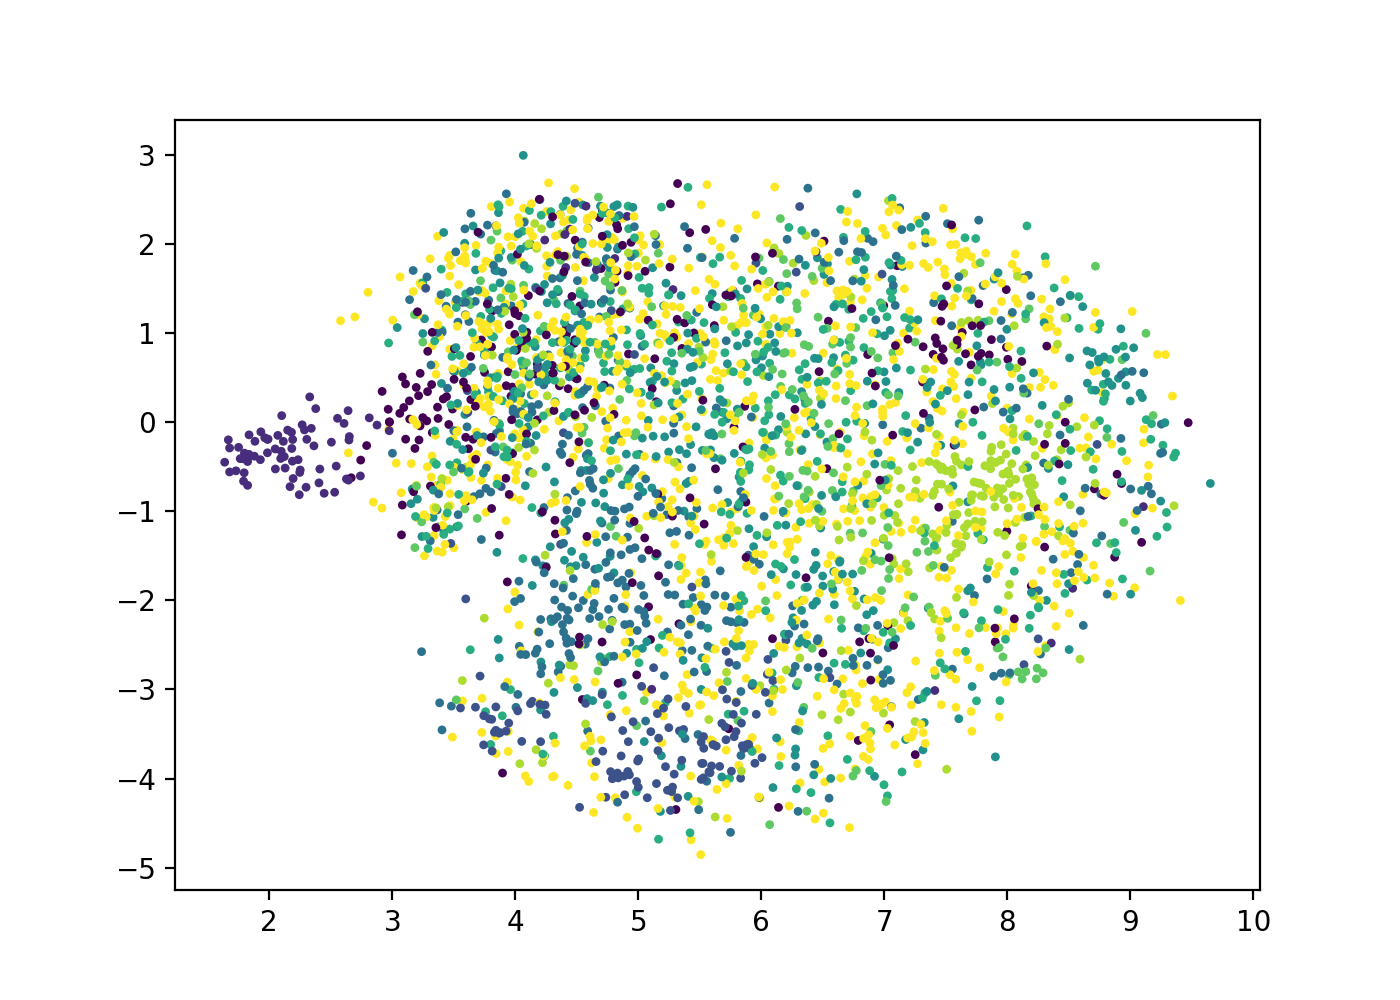
\includegraphics[width=.9\linewidth]{km-no-lsa.png}	
%		\caption{\label{fig:km-no-lsa.png}K-Means without LSA Cluster Figure } 
%	\end{minipage}\hfill
%	
%\end{figure}

\subsubsection{K-Means Clustering with LSA}
%\begin{figure}[!htb]
%	\begin{minipage}{\textwidth}
%		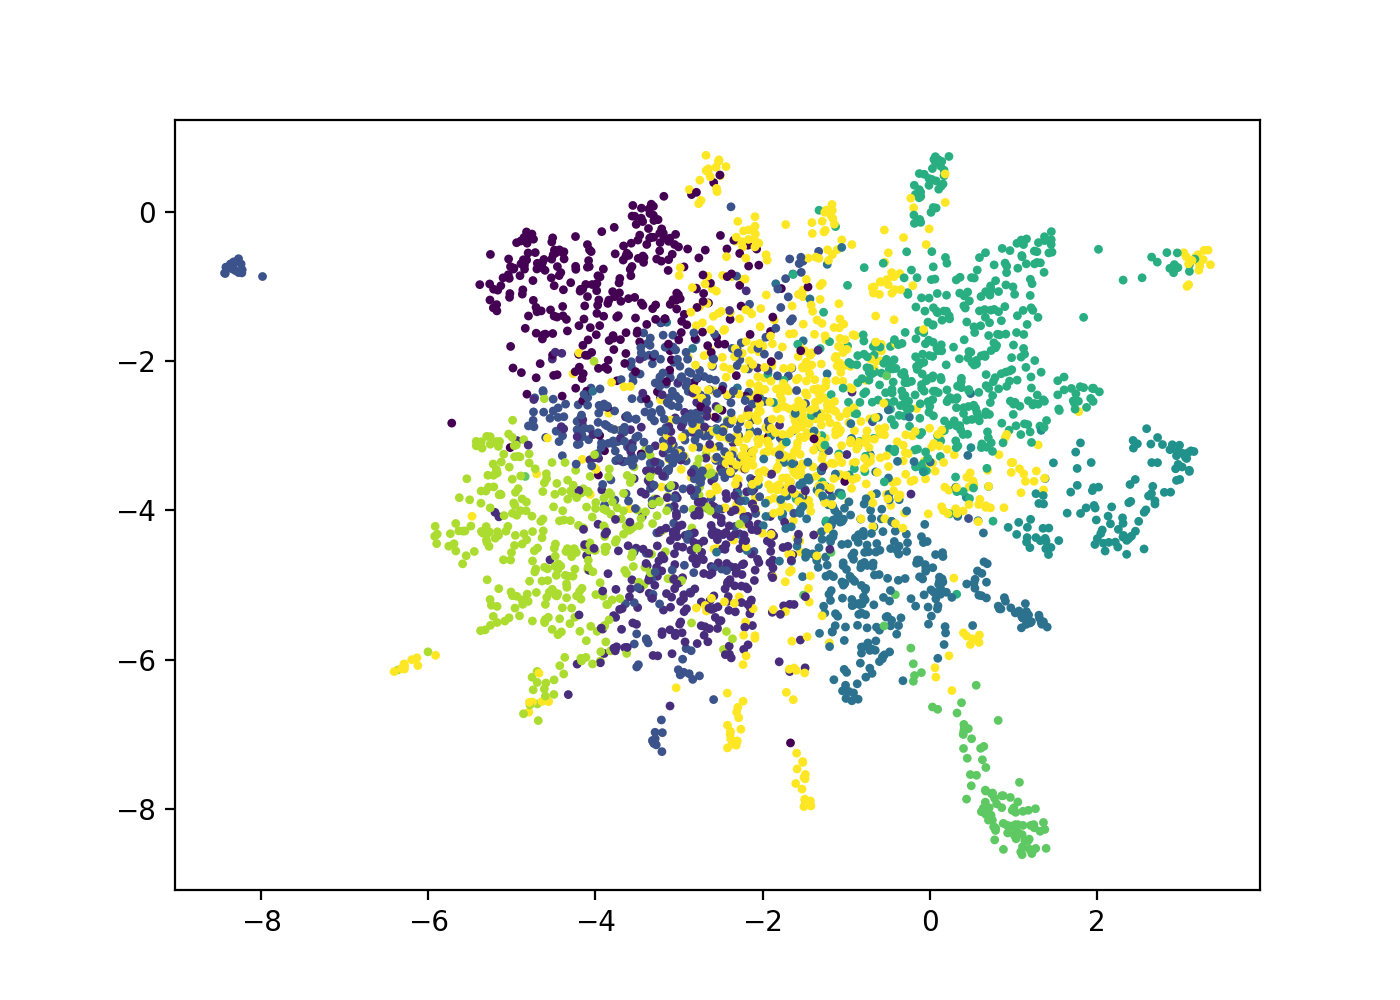
\includegraphics[width=.9\linewidth]{lsa}	
%		\caption{\label{fig:lsa}K-Means with LSA Cluster Figure } 
%	\end{minipage}\hfill
%	
%\end{figure}

The program can be run using the following command for K-Means clustering:
\begin{lstlisting}[frame=none]
$python document-clustering.py kmeans-lsa
\end{lstlisting}
The running result:
\begin{lstlisting}[frame=single, captionpos=b, caption=Silhouette Score List, label=listing:sparql_getallindividuals,]
Cluser Number: 2  silhouette_score: 0.0254
Cluser Number: 3  silhouette_score: 0.03
Cluser Number: 4  silhouette_score: 0.0334
Cluser Number: 5  silhouette_score: 0.0391
Cluser Number: 6  silhouette_score: 0.0385
Cluser Number: 7  silhouette_score: 0.0411
Cluser Number: 8  silhouette_score: 0.0441
Cluser Number: 9  silhouette_score: 0.0484
Cluser Number: 10  silhouette_score: 0.0459
\end{lstlisting}
We select cluster number: 9, which has the highest silhouette score. We can have all clusters with the top 8 topics listed as following.
\begin{lstlisting}[frame=single, captionpos=b, caption=LSA Cluster Result, label=listing:sparql_getallindividuals,]
Cluster 0: power like circuit chip output need ground using
Cluster 1: graphics files file image program format package color
Cluster 2: space nasa moon launch earth shuttle orbit lunar
Cluster 3: people jesus religion article believe think bible christian
Cluster 4: article know think like time science question long
Cluster 5: pitt banks gordon chastity intellect skepticism surrender cadre
Cluster 6: food doctor disease pain medical patients people cause
Cluster 7: objective morality moral keith frank caltech livesey values
Cluster 8: thanks information looking mail know advance info help
\end{lstlisting}
We visualize the clusters, which helps to distinguish the document cluster distribution, see Figure~\ref{fig:lsa}.

\begin{figure}[!htb]
	\begin{minipage}[b]{0.5\textwidth}
		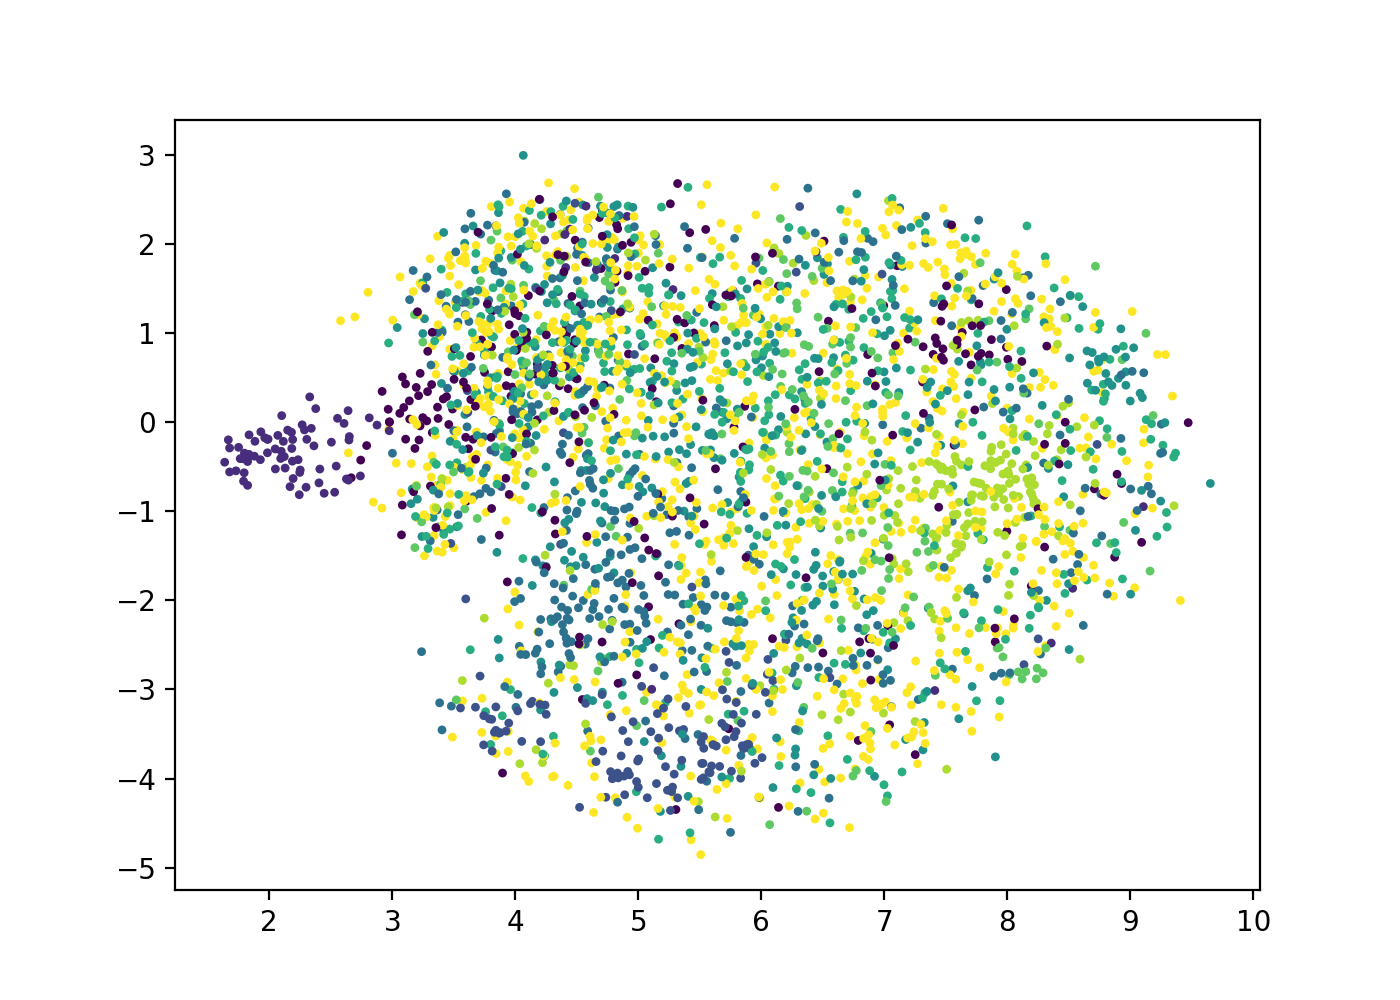
\includegraphics[width=.9\linewidth]{km-no-lsa}	
		\caption{K-Means without LSA} 
		\label{fig:km-no-lsa}
	\end{minipage}\hfill
	\begin{minipage}[b]{0.5\textwidth}
		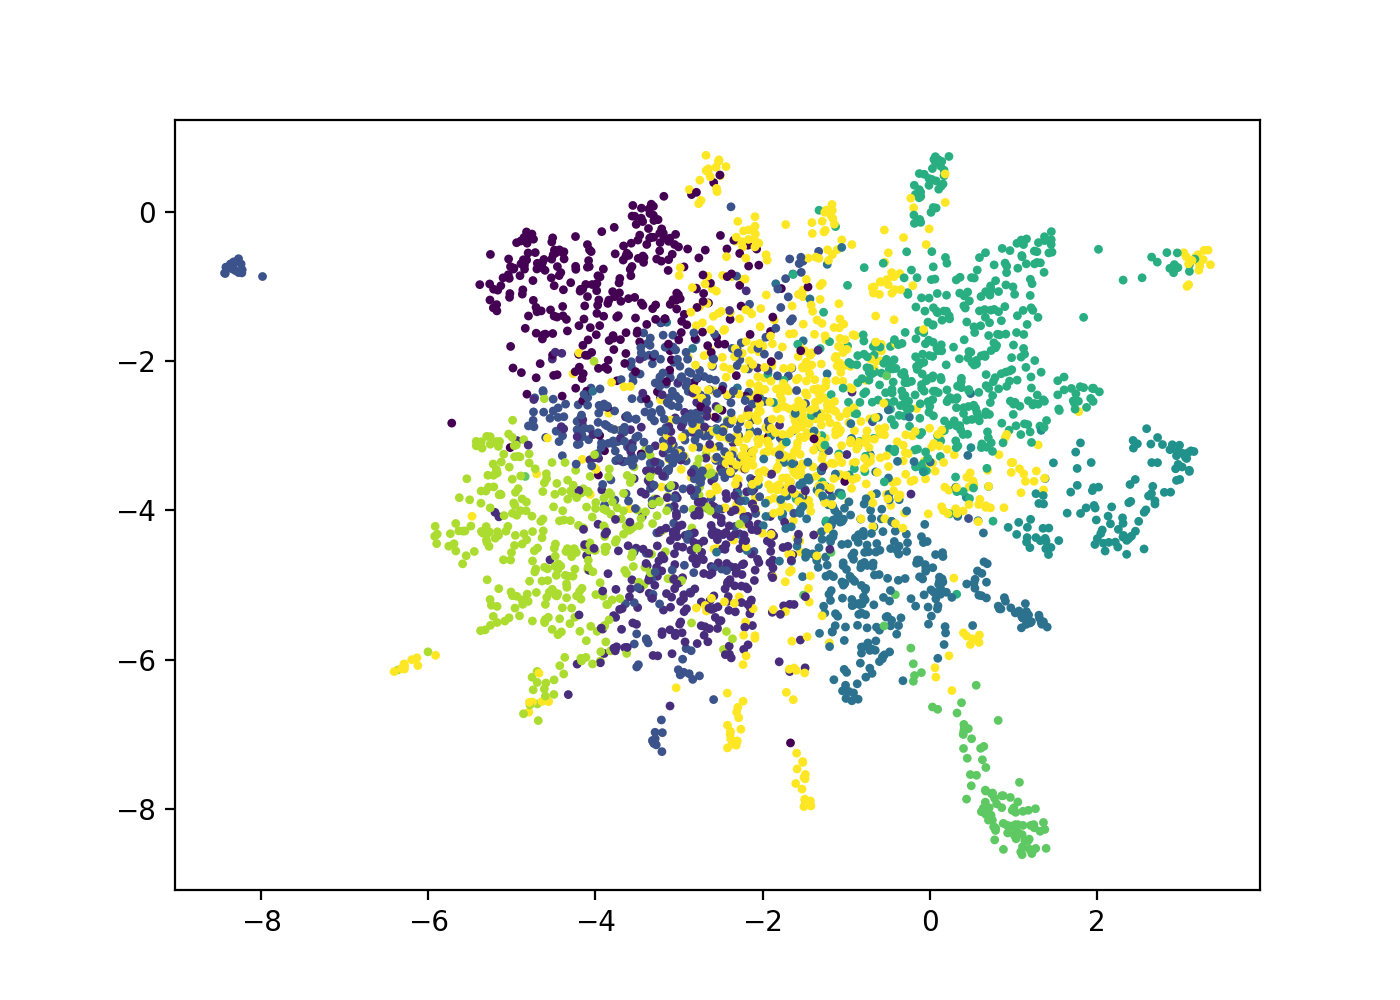
\includegraphics[width=.9\linewidth]{lsa}	
		\caption{K-Means with LSA} 
		\label{fig:lsa}
	\end{minipage}
\end{figure}

\subsubsection{Topic Modeling Clustering with LDA}
The program can be run using the following command for topic modeling clustering:
\begin{lstlisting}[frame=none]
$python document-clustering.py lda
\end{lstlisting}
The running result:
\begin{lstlisting}[frame=single, captionpos=b, caption=Coherence Score List, label=listing:sparql_getallindividuals,]
Cluster Number: 2  Coherence Value: 0.3374
Cluster Number: 3  Coherence Value: 0.3631
Cluster Number: 4  Coherence Value: 0.3486
Cluster Number: 5  Coherence Value: 0.41
Cluster Number: 6  Coherence Value: 0.3557
Cluster Number: 7  Coherence Value: 0.3732
Cluster Number: 8  Coherence Value: 0.3592
Cluster Number: 9  Coherence Value: 0.3716
Cluster Number: 10  Coherence Value: 0.3577
\end{lstlisting}
We select cluster number: 7, which has the highest coherence score. We print out the top 8 topics for each cluster, the output 
\begin{lstlisting}[frame=single, captionpos=b, caption=Topic Modeling Cluster Result, label=listing:sparql_getallindividuals,]
Cluster 0: would writes article like used need power ground  
Cluster 1: image graphics file writes jpeg files system would  
Cluster 2: would writes people article think like know time  
Cluster 3: pain pitt gordon article bank  patients writes candida  
Cluster 4: space nasa data also informatio launch research program  
Cluster 5: jesus bible christian believe christians writes christ article  
Cluster 6: sandvik compass apple kent tyre mwra newton rows  
\end{lstlisting}


\section{Conclusions} 
In this project, we have experiments using three clustering models, we present that LSA can be used to cluster documents into different groups according to their topics, and in each cluster the top topics are highly related, LSA can provide high internal cluster similarity. For basic K-Means clustering without LSA, the silhouette scores are lower than the one with LSA, which means the cluster quality with LSA is better, this can be concluded from the cluster visualization as well. In topic modeling with LDA, we evaluate the cluster quality through coherence score, which helps us to decide the optimal number of topics. Through building LDA model on the clean dataset, we can obtain the clustering result.  
\par

We have to consider the fact that we use small dataset, only 3219 documents. This work can be extended by using a larger document collection with more topics. We only compare the cluster performance between K-Means with and without LSA, in the future we will evaluate the performance for both K-Means with LSA and topic modeling clustering to see which one performs better.



%\clearpage
\begin{thebibliography}{9}

\bibitem{textbook}
Daniel Jurafsky and James H. Martin. Speech and Language Processing: An
Introduction to Natural Language Processing, Computational Linguistics,
and Speech Recognition. Second Edition 2009.

\bibitem{Intro} 
Thomas K Landauer, Peter W.Foltz and Darrell Laham. 
\textit{An introduction to latent semantic analysis}. Discourse Process. 1998.

\bibitem{lda} 
David M. Blei, Andrew Y. Ng, and Michael I. Jordan. Latent Dirichlet allocation. JMLR, 3, 2003.

\bibitem{news} 
\textit{http://qwone.com/~jason/20Newsgroups/}. 20Newsgroups.



\end{thebibliography}


\end{document}